\documentclass[10pt]{article}
\usepackage[hmargin={.5in},vmargin={.5in},foot={.6in}]{geometry}   
\geometry{letterpaper}              
\usepackage{color,graphicx}
\usepackage{setspace}
\usepackage{amsmath}
\usepackage{amssymb}
\usepackage{varioref}
\usepackage{textcomp}
\usepackage{textcomp}
\usepackage{mflogo}
\usepackage{wasysym}
\usepackage[normalem]{ulem}
\usepackage{hyperref}
\usepackage{booktabs}
\usepackage{natbib}

\newcommand{\HRule}{\rule{\linewidth}{0.25mm}}

\usepackage{fancyhdr} % This should be set AFTER setting up the page geometry
\pagestyle{plain} % options: empty , plain , fancy
\lhead{}\chead{}\rhead{}
\renewcommand{\headrulewidth}{.5pt}
\lfoot{}\cfoot{\thepage}\rfoot{}
\newcommand{\txtp}{\textipa}
\renewcommand{\rm}{\textrm}
\newcommand{\sem}[1]{\mbox{$[\![$#1$]\!]$}}
\newcommand{\lam}{$\lambda$}
\newcommand{\lan}{$\langle$}
\newcommand{\ran}{$\rangle$}
\newcommand{\type}[1]{\ensuremath{\left \langle #1 \right \rangle }}

\newcommand{\bex}{\begin{exe}}
\newcommand{\eex}{\end{exe}}
\newcommand{\bit}{\begin{itemize}}
\newcommand{\eit}{\end{itemize}}
\newcommand{\ben}{\begin{enumerate}}
\newcommand{\een}{\end{enumerate}}

\newcommand{\gcs}[1]{\textcolor{blue}{[gcs: #1]}}
\definecolor{Green}{RGB}{10,200,100}
\newcommand{\ndg}[1]{\textcolor{Green}{[ndg: #1]}}


\thispagestyle{plain}

\title{Subjectivity predicts adjective ordering preferences}
%\author{Gregory Scontras, Judith Degen, Noah D.~Goodman}
%\date{}

\begin{document}

%\maketitle

\begin{center}
	\textbf{Subjectivity predicts adjective ordering preferences}
\end{center}
From English to Hungarian to Mokilese, speakers exhibit strong ordering preferences in multi-adjective strings: ``the big blue box'' sounds far more natural than ``the blue big box.'' We show that an adjective's distance from the modified noun is predicted not by a rigid syntax, but by the adjective's meaning: less subjective adjectives occur closer to the nouns they modify.  
We believe that subjectivity synthesizes---rather than supplants---many of the previous approaches to adjective ordering, incorporating notions like ``inherentness'' and ``context dependence'' into an intuitive psychological construct that readily operationalizes as a behavioral measure. 
	We established two empirical constructs: the preferences themselves, which we measured using naturalness ratings and validated with corpus statistics; and adjective subjectivity, which we measured directly and corroborated with potential for faultless disagreement. 
An adjective's semantics predicts its distance from the modified noun, such that less subjective adjectives occur linearly closer to nouns they modify. XXX REFERENCE TO FIGURES.
To evaluate the \emph{relative} success of subjectivity, we investigated the predictions of three other hypotheses from the literature: adjective inherentness (i.e., how essential an adjective's meaning is to the noun it modifies; \citealp{sweet1898,whorf1945}), intersective vs.~subsective modification (i.e., the mode by which an adjective composes semantically with the noun it modifies; \citealp{truswell2009}), and concept formability (i.e., whether an adjective composes with a noun to form a complex, idiomatic concept; \citealp{McNally2004,bouchard2005,svenonius2008}). In each case, we found that subjectivity has greater predictive power.
	While subjectivity accounts for the regularities we observe in adjective ordering, the deeper explanation for how subjectivity determines the relative order of adjectives remains unsettled. Our results suggest that ordering preferences likely emerge, at least partially, from a desire to place less subjective content closer to the substantive head of a nominal construction (i.e., closer to the modified noun). 
Subjective content allows for miscommunication to arise if speakers and listeners arrive at different judgments about a property description. Hence, less subjective content is more useful at communicating about the world. 
An explanation along these lines, based on pressures to facilitate successful reference resolution, would have to depend on the hierarchical, not linear, ordering of adjectives: noun phrases are built semantically outward from the noun, and more useful, less subjective content enters earlier in this process (cf.~the mirroring of preferences in pre- vs.~post-nominal languages). 
Whatever its source, the success of subjectivity in predicting adjective ordering preferences provides a compelling case where linguistic universals, the regularities we observe in adjective ordering, emerge from cognitive universals, the subjectivity of the properties that the adjectives name.

\noindent\begin{minipage}{.32\textwidth}
	%\begin{figure}
		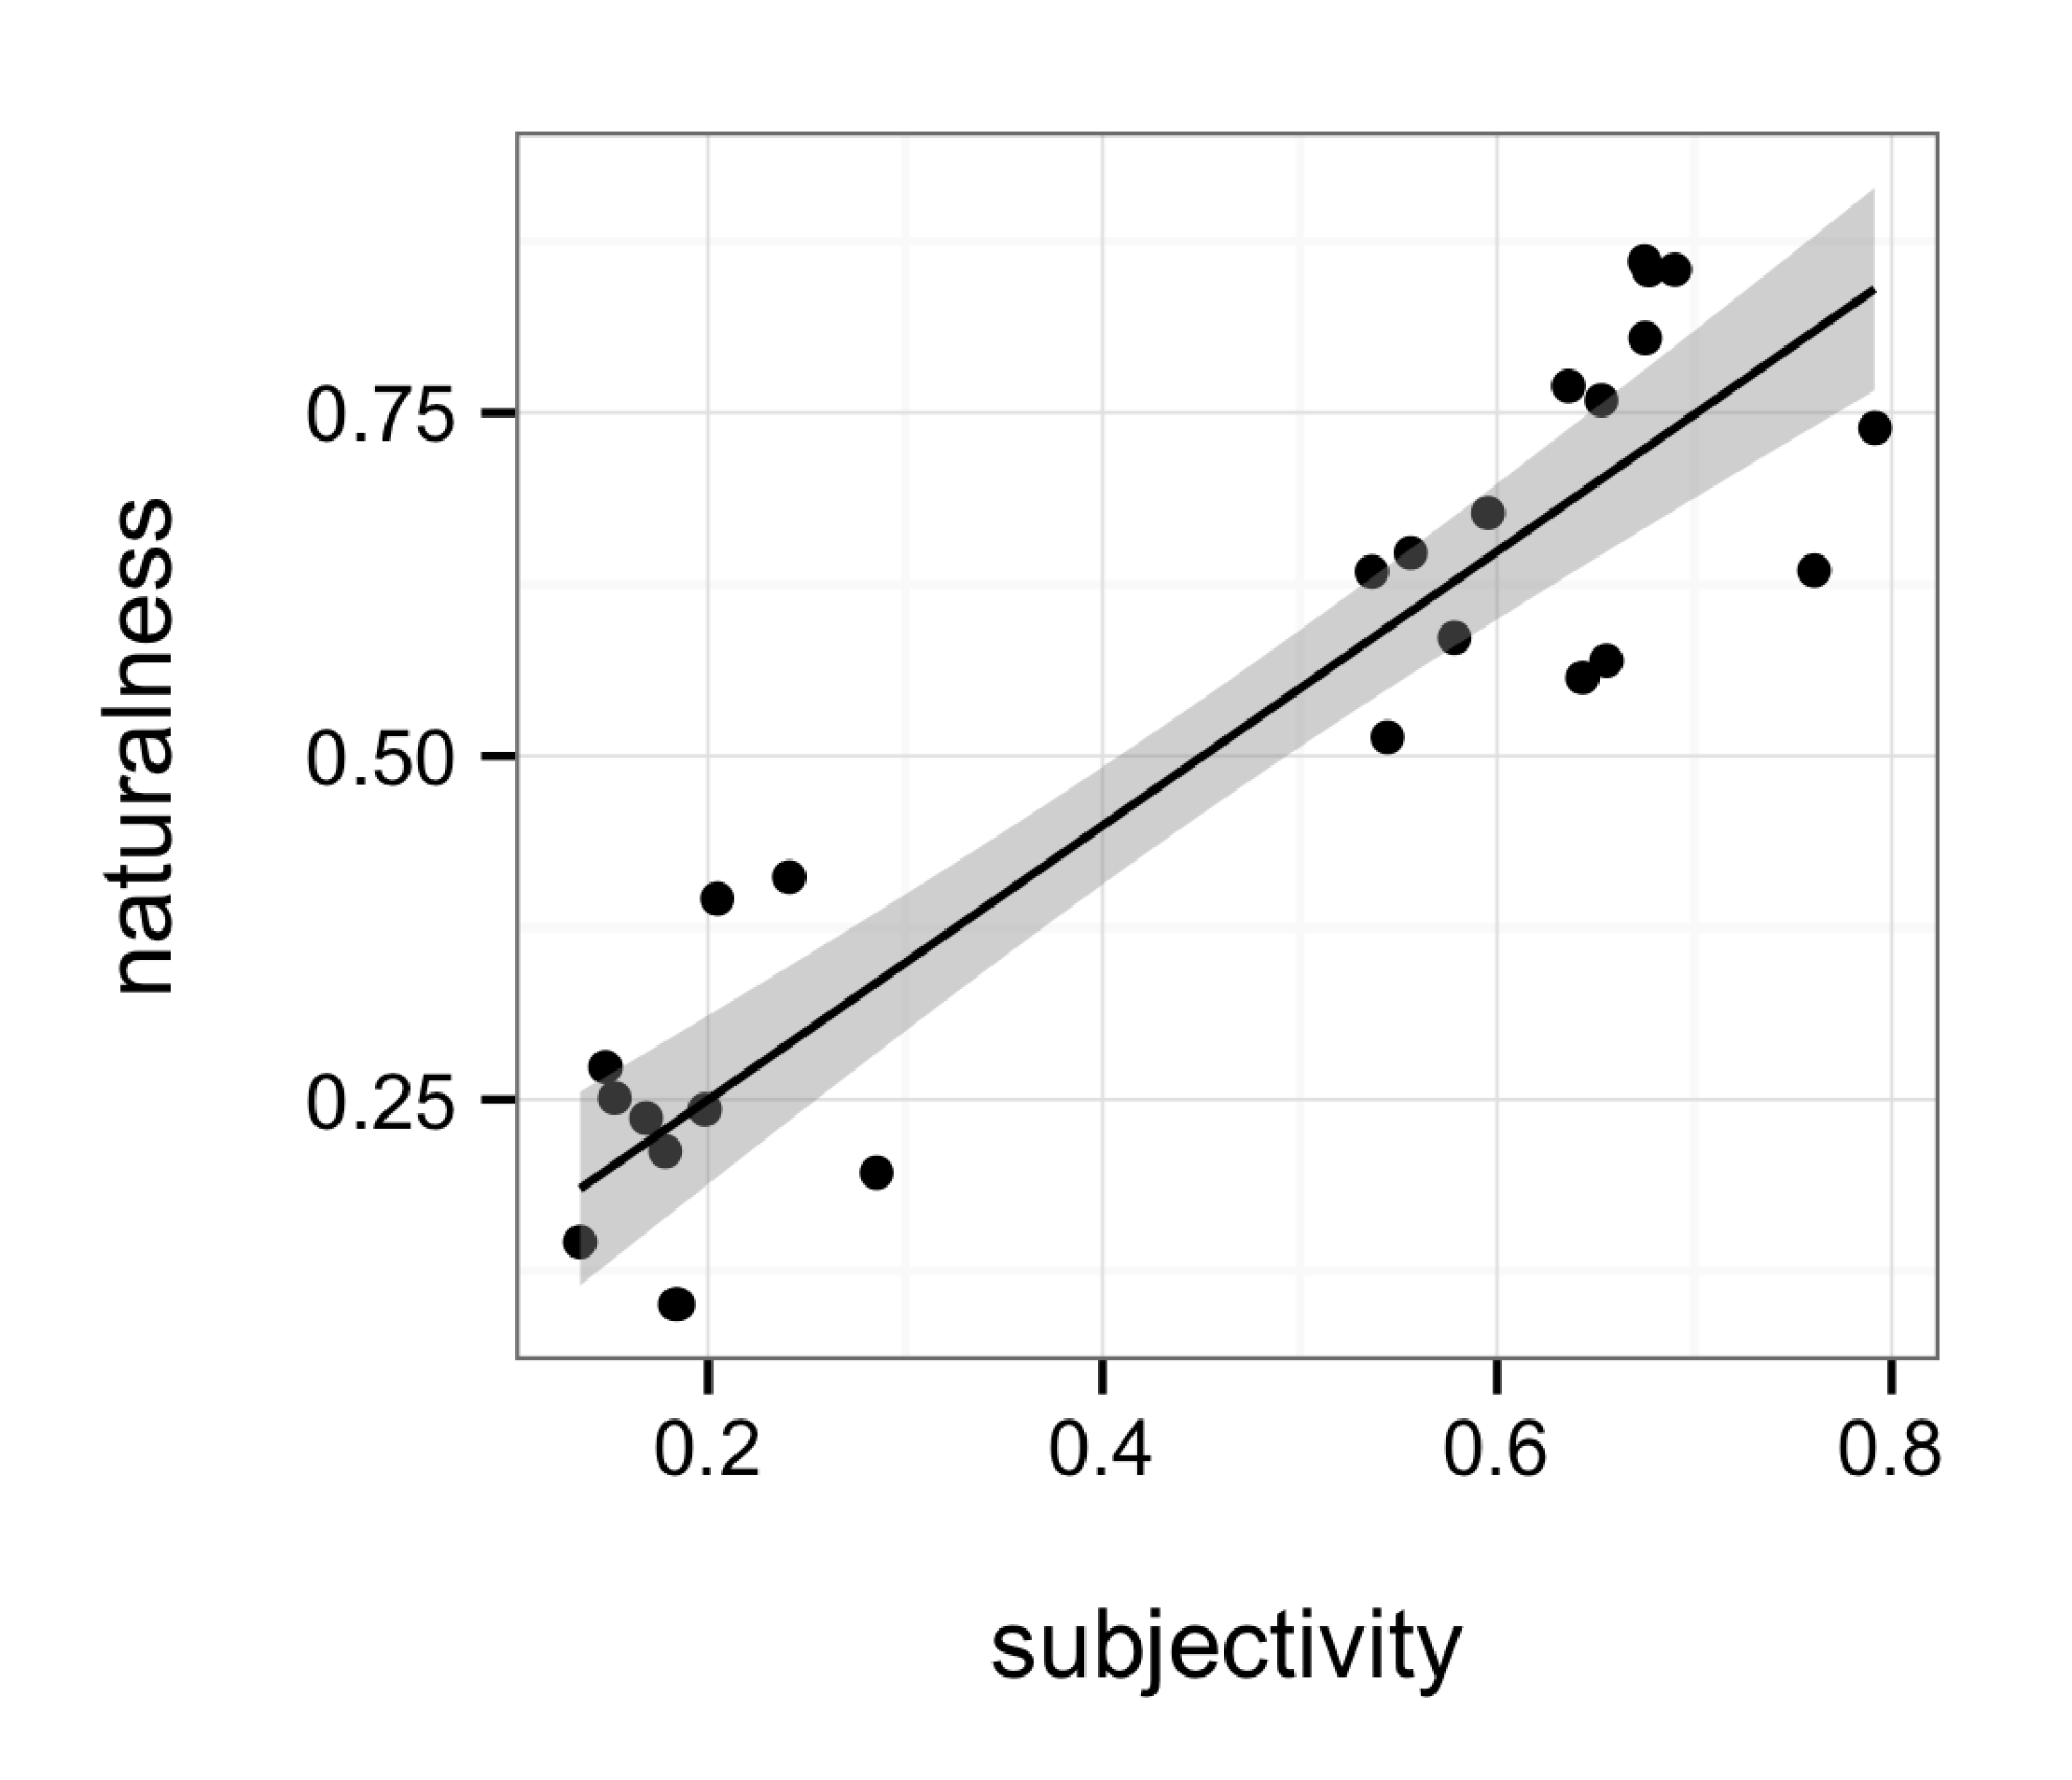
\includegraphics[width=.95\linewidth]{plots/naturalness-subjectivity-new.eps}\\
		\includegraphics[width=.95\linewidth]{plots/expt3_nat-sub.eps}
		%\caption{
		Fig.~1: Mean naturalness ratings plotted against mean subjectivity scores for each of the adjectives tested in Expt.~1. (top) and Expt.2 (bottom). Superlatives are labeled in green; outlier adjectives are labeled in blue.
		%}\label{naturalness-subjectivity-pred}
	%\end{figure}
\end{minipage} 
\begin{minipage}{.32\textwidth}
	%\centering
	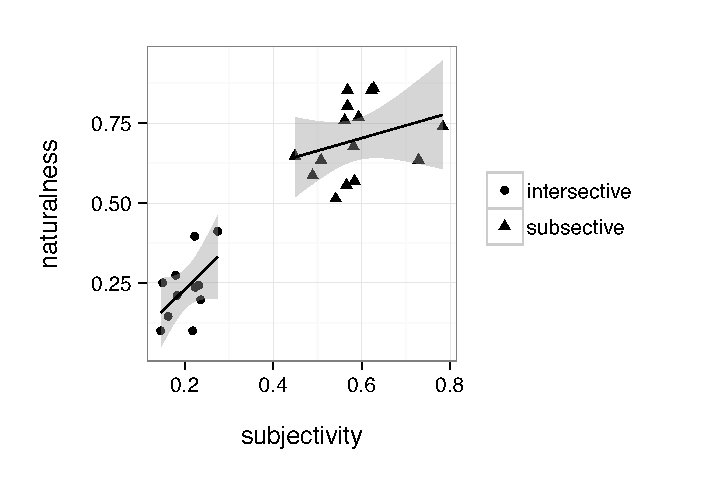
\includegraphics[width=.95\linewidth]{plots/expt1-subjectivity-subsectivity.eps}\\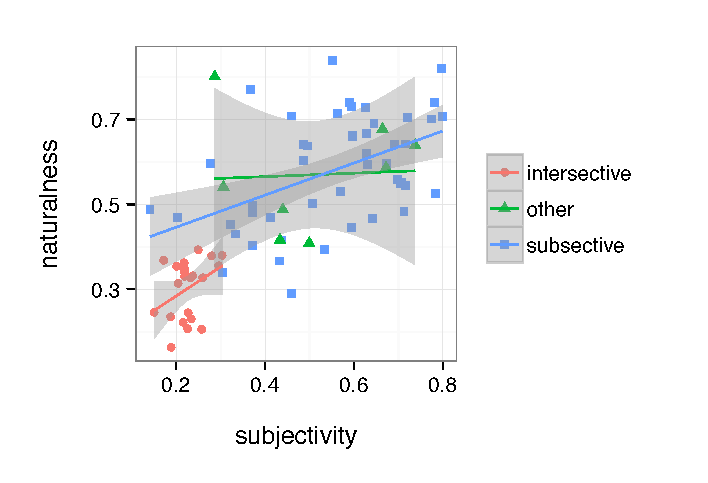
\includegraphics[width=.95\linewidth]{plots/expt3-subjectivity-subsectivity.eps}
	%\caption{
	Fig.~2: Mean naturalness ratings plotted against mean subjectivity scores grouped by subsectivity for the adjectives tested in Expt.~1 (\emph{top}) and in Expt.~2 (\emph{bottom}).
		%}\label{fig:subsectivity}
\end{minipage} 
\begin{minipage}{.32\textwidth}
	%\centering
	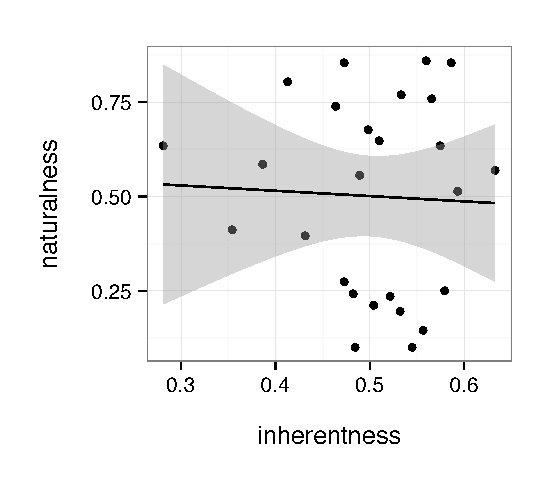
\includegraphics[width=.95\linewidth]{plots/expt1-inherentness-naturalness.eps}%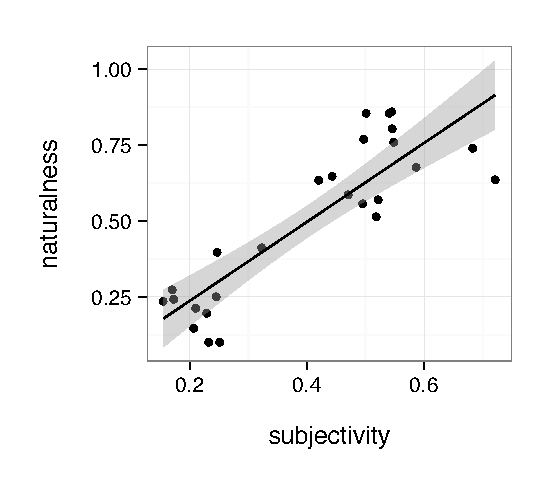
\includegraphics[width=3in]{plots/expt1-subjectivity2-naturalness.eps}	
	\\
	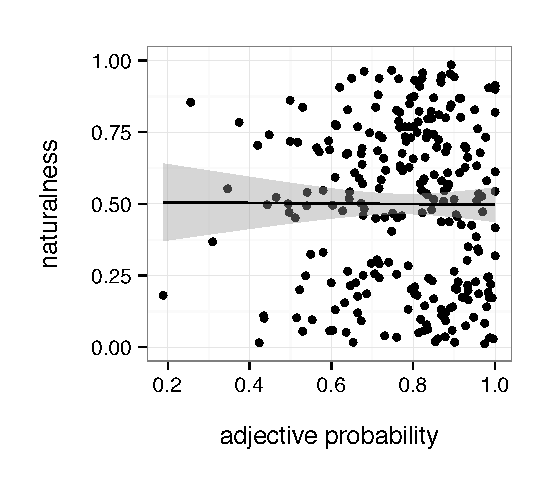
\includegraphics[width=.95\linewidth]{plots/naturalness-concept-noun-pred.eps}
	%\caption{
	Fig.~3: TOP: Mean naturalness ratings plotted against mean inherentness  %(\emph{left}) and subjectivity (\emph{right}) 
	(top) and concept-formability (bottom) scores for each of the adjectives tested
	in Expt.~1. Concept-formability scores take into account specific noun information.
	%	}\label{fig:inherentness}
\end{minipage}

%
%\begin{figure}
%	\centering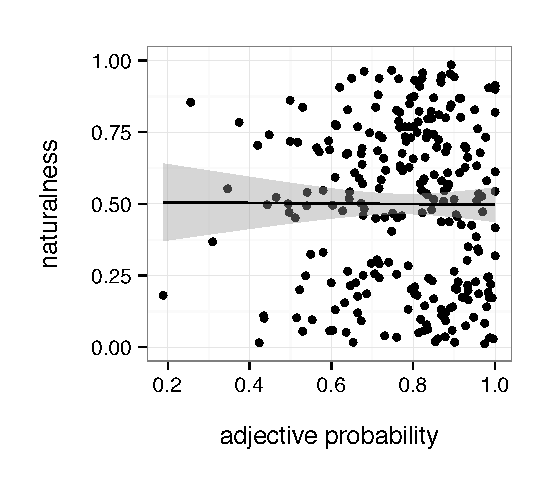
\includegraphics[width=3in]{plots/naturalness-concept-noun-pred.eps}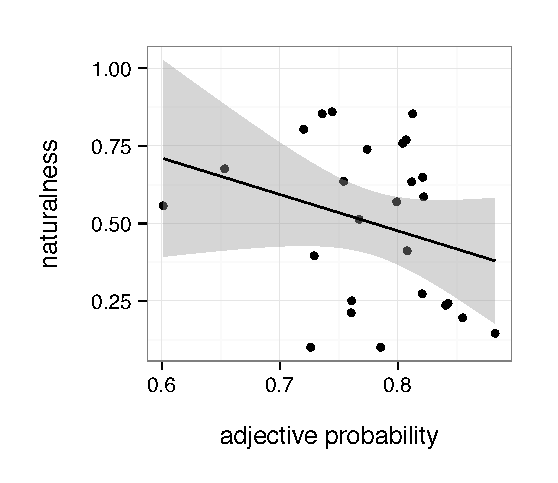
\includegraphics[width=3in]{plots/naturalness-concept-adjective.eps}
%	\caption{Mean naturalness ratings plotted against mean adjective probability (i.e., concept-formability) scores for each of the 26 adjectives tested. In computing mean adjective probability, we either took into account (\emph{left}) or collapsed over (\emph{right}) specific noun information.}\label{fig:concept}
%\end{figure}

\newpage

  \bibliographystyle{chicago} 
  \bibliography{adjectives}


\end{document}














